% \iffalse
% This is textpos.dtx, which allows you to place text (and graphics)
% anywhere on the LaTeX page.  It's useful for posters.
%
%%%% File: textpos.dtx
%%%% Copyright 1999, 2001-03, 2005-7, 2009-12, 2014-16., Norman Gray
%%
%% This work may be distributed and/or modified under the
%% conditions of the LaTeX Project Public License, either version 1.3
%% of this license or (at your option) any later version.
%% The latest version of this license is in
%%   http://www.latex-project.org/lppl.txt
%% and version 1.3 or later is part of all distributions of LaTeX
%% version 2005/12/01 or later.
%%
%% This work has the LPPL maintenance status `maintained'.
%%
%% The Current Maintainer of this work is Norman Gray <http://nxg.me.uk>
%%
%% This work consists of the files textpos.dtx and textpos.ins,
%% and the derived file textpos.cls.
%%
%% Author: Norman Gray, norman@astro.gla.ac.uk.
%% Department of Physics and Astronomy, University of Glasgow, UK
%%
%% See the file LICENCE for a copy of the LPPL.
%%
%% Mercurial ident: 8aa202e2b283, 2016-06-07 23:52 +0100
%%
%<+package>\NeedsTeXFormat{LaTeX2e}
%<+package>\ProvidesPackage{textpos}[2016/06/07 v1.8]
%<+package>\typeout{Package: textpos 2016/06/07 1.8, absolute positioning of text on the page}
%
%<*driver>
\documentclass{ltxdoc}
\title{Textpos: absolute positioning of text on the page}
\author{Norman Gray\\(\texttt{http://nxg.me.uk})}
\date{Version 1.8, 2016 June 7\footnote{Mercurial ident: 8aa202e2b283, 2016-06-07 23:52 +0100.
This software is copyright, 1999, 2001-03, 2005-7, 2009-12, 2014-16. Norman Gray.
It is released under the terms of the LaTeX Project Public License,
either version 1.3 of this licence or (at your option) any later version.
The latest version of this license is at \texttt{http://www.latex-project.org/lppl.txt}.}}
\newcommand\Lopt[1]{\textsf {\small [#1]}}
\newcommand\file[1]{\texttt {#1}}
\newcommand\Lcount[1]{\textsl {\small#1}}
\newcommand\Lenv[1]{\texttt{\{#1\}}}
\newcommand\pstyle[1]{\textsl {#1}}
\makeatletter % make the ttfamily font less overbearingly large
\renewcommand\ttfamily{\not@math@alphabet\ttfamily\mathtt
    \fontfamily\ttdefault
    \fontsize{9}{\f@baselineskip}\selectfont}
\makeatother
% Make command strings easier to write
\def\activemeta#1>{\meta{#1}}
{\catcode`\<=\active
 \gdef\cmd{\begingroup
   \catcode`\\=12 \catcode`\{=12 \catcode`\}=12
   \catcode`\<=\active \let<\activemeta
   \catcode`\|=12
   \docmd}}
\def\docmd|#1|{\texttt{#1}\endgroup}
%% \url macro (url.sty does this better)
\def\setpathdots{\discretionary{.}{}{.}}
\def\setpathslash{\discretionary{/}{}{/}}
{\catcode`\.=\active
 \catcode`\/=\active
  \gdef\pathcats{%
    \catcode`\%=12      \catcode`\~=12
    \catcode`\.=\active  \let.\setpathdots
    \catcode`\/=\active \let/\setpathslash
    \catcode`\#=12      \catcode`\_=12}%
    }
\def\setpath#1{\ttfamily\small <\nobreak #1\nobreak>\endgroup}
\def\url{\begingroup\pathcats\setpath}
%\RecordChanges
%\OnlyDescription
\begin{document}
\maketitle
\tableofcontents
%% \bigskip
%% \hrule
%% \bigskip
\newpage
\DocInput{textpos.dtx}
\end{document}
%</driver>
%
% \fi
%
%
%
%
% \changes{v1.0a}{1998/04/29}{Robin Fairbairns pointed out and adjusted errors in the documentation}
% \changes{v1.0b}{1998/04/30}{Reorganised documentation -- properly this time}
% \changes{v1.1b}{1999/03/05}{Added note to the effect that everyshi can be found at CTAN}
% \changes{v1.1c}{1999/03/09}{Corrected checksum (again!)}
% \changes{v1.1d}{1999/06/06}{Clarified copyright and licence status}
% \changes{v1.3?}{2003/06/??}{Finally removed bloody useless checksum and character table}
%
%
% \noindent
% This package facilitates placing boxes at absolute positions on the
% \LaTeX\ page.  There are several reasons why this might be useful, but
% the reason which originally motivated this package is to help produce a
% large-format conference poster.  However the facility is also useful
% for filling in forms or other special purpose layout.
%
% This package provides a single environment, which contains the text
% (or graphics, or table, or whatever) which is to be placed on the
% page, and which specifies where it is to be placed.
%
% The package tries not to get in the way.  That is, you should be
% able to use most of the apparatus of \LaTeX\ in your poster, such as
% section headings, citations, graphics inclusion, and so on.  Please
% let me know if you experience problems in this respect.
%
% This package requires the services of Martin Schr\"oder's package
% \texttt{everyshi}.  If this is not already part of your \TeX{}
% installation, you will need to download this package from CTAN.  See
% \url{http://www.tex.ac.uk/tex-archive/macros/latex/contrib/supported/ms/}
% or one of the other CTAN hosts.
%
% Textpos has a home page at \url{http://purl.org/nxg/dist/textpos}.
% The source is held at bitbucket: \url{https://bitbucket.org/nxg/textpos},
% and there is an issues list there, for bug reports.  Code
% contributions or fixes are welcome, but note that I feel that
% Textpos is pretty mature now, and I'm reluctant to extend its
% functionality beyond its natural boundaries, so it would be wise to
% chat to me about any new features before spending a lot of time
% drafting them in code.
%
% An article describing Textpos appeared in TUGboat in 2002:
% Norman Gray, `Absolute Positioning with
% Textpos', TUGboat \textbf{23} (3/4), pp341--4, 2002, available at
% \url{http://www.tug.org/TUGboat/tb23-3-4/tb75gray.pdf}.
%
% \section{Description}
%
% Load the package as usual, with
% \begin{quote}
% \cmd|\usepackage<package-options>{textpos}|
% \end{quote}
% The \meta{package-options} are as described in section~\ref{packopts}.
%
% The environment is used as follows
% \DescribeEnv{textblock}
% \begin{quote}\begin{raggedright}
% \cmd|\begin{textblock}{<hsize>}(<hpos>,<vpos>)|\\
% text...\\
% |\end{textblock}|
% \end{raggedright}
% \end{quote}
% The \meta{hsize} and \meta{hpos} arguments are given in units of a
% module |\TPHorizModule|, and \meta{vpos} is given in units of a
% module |\TPVertModule|.  You set these using
% the command
% \cmd|\setlength{\TPHorizModule}{<dimen>}|,
% and similarly for |\TPVertModule|.
% The arguments may be any dimension, and you may use the modules as
% units elsewhere in your document if you wish to, for example in
% \texttt{\bslash makebox[2\bslash TPHorizModule]\{gnus\}}.  The text in the
% environment will be set in a
% box \meta{hsize} modules wide, and placed on the page with its
% upper left corner at the position (\textit{hpos,vpos}).  As is
% natural in \TeX, the \meta{vpos} parameter indicates distance
% \emph{down} from the `anchor point' (see below).
%
% The \Lenv{textblock} parameters \meta{hsize},
% \meta{hpos} and \meta{vpos} are \emph{multiples or fractions of the horizontal
% and vertical modules}, as appropriate.  If you want or need to give
% explicit sizes here, see the \Lenv{textblock*} environment below.
%
% Notice that the positioning arguments for the \Lenv{textblock}
% command -- the coordinates \cmd|...(<hpos>,<vpos>)| -- are in
% \emph{round} brackets,\marginpar{Round brackets!}
% not curly ones.  This is in imitation of the \texttt{picture}
% environment, and whether or not this is sensible, it's not going to
% change now.
%
% This package works in two modes, relative and absolute.
% \marginpar{relative \& absolute mode}
% In the first one, the default, the block-positioning parameters in the
% \Lenv{textblock} envirionment are taken to be relative to an `anchor
% point' which is the current position on the page, that is, the place
% where (the bottom left of) a character would appear if it were typed
% at this point.  This will be appropriate if you are
% laying out text within a \texttt{figure} environment or the like.
% In this mode, you will typically give several \Lenv{textblock}
% environments one after the other, so that they are all relative to
% the same point.
%
% If, however, your entire
% document is to be laid out piece by piece (which is the case in the
% canonical use of the package, to lay out a poster), then you might
% want to be more sure of where the origin is.  In this case, you make
% the package work in its absolute mode, by invoking it with
% the \Lopt{absolute} option: |\usepackage[absolute]{textpos}|.
% In this mode, all the block-positioning parameters are given
% relative to a single origin on the page.  By default, this `anchor point' is the
% top-left corner of the page, but you may change it with the
% command \cmd|\textblockorigin{<hpos>}{<vpos>}|.
% Here \meta{hpos} and \meta{vpos} are dimensions such as `10mm',
% relative to the top-left corner of the paper.  You may use this
% command only if the package was invoked with the \Lopt{absolute}
% option.  See also section~\ref{packopts} for how to alternate
% between modes, and section~\ref{absolute-newpage} for notes on the
% interaction with the |\newpage| command.
%
% The textblocks are placed on the page in the order in which they
% appear in the file.  This means that later textblocks will be placed
% on top of earlier ones, which may matter if one or other contains,
% for example, a block of opaque colour (I believe this to be true in
% practice for all output mechanisms, though I doubt it's guaranteed
% in principle).  This order was unspecified before textpos 1.7e; it
% was changed, and specified, in that version.
%
% The \Lenv{textblock} environment will most often be used in
% vertical mode.  If it is called in horizontal (ie, paragraph) mode,
% however, it will silently create a paragraph break by inserting a
% |\par| command before the environment; it remains in vertical mode
% after the environment is finished.  It should have no further
% effects on spacing, and if you find that it does, that's a bug.  If
% you try to use the environment when in maths mode, the package
% objects (as it should!).
%
% \subsection{Package options}
% \label{packopts}
%
% There are several package options:
% \begin{description}
% \item[\Lopt{showboxes}]When you are laying things out, it can be
% useful to have the boxes drawn in for you.  This option draws a box
% fitting closely round the set text.
% \item[\Lopt{noshowtext}]This suppresses the display of the text in
% each block (so it's not really usable without the \Lopt{showboxes}
% option).  The resulting box will be the correct size, but empty,
% unless the |\textblocklabel| command has been given.  This
% can be useful when you are previewing a document.
% \item[\Lopt{absolute}]If this is present, then the positions on the
% \Lenv{textblock} environment are taken to be absolute positions on
% the page.  See above for more detail, and see
% section~\ref{absolute-newpage} for the interaction with the
% |\newpage| command.  There is also a \Lopt{relative} option, but
% since relative mode is, and will remain, the default, the
% \Lopt{relative} option is redundant, and is here only for symmetry.
% \item[\Lopt{overlay}]When using the absolute-position mode, the
% textblocks are placed under any other text on the page.  This is
% normally what you want, but if you have page contents, and they have
% something
% which \emph{obscures} the textblocks (for example, a block of opaque
% colour), then the positioned textboxes disappear.  In this case,
% specify the option \Lopt{overlay}, to request that the positioned
% blocks of text overlay any other page contents, rather
% than being overlaid.
% \item[\Lopt{verbose}, \Lopt{quiet}]The package writes a few messages
% to the output, describing its calculations.  These are potentially
% irritating, so you can turn them off with the \Lopt{quiet} option or
% on with the \Lopt{verbose} option.  The default is currently
% \Lopt{verbose}, but this might change in future.
% \end{description}
%
% \subsection{Changing options on the fly}
% \label{s:changing-options}
%
% \begin{macro}{\TPoptions}
% Each of the options mentioned in the previous section can be changed within the body of the text,
% using the command |\TPoptions| with a comma-separated list of
% keywords
% \textit{$\langle$keyword$\rangle$}\texttt{=true} or
% \textit{$\langle$keyword$\rangle$}\texttt{=false}.
% The recognised keywords are `absolute', `overlay', `verbose',
% `showboxes' and `showtext'.  Thus the command
% \begin{quote}
% |\TPoptions{absolute=false , showboxes = true }|
% \end{quote}
% will switch off \Lopt{absolute} mode, and switch on \Lopt{showboxes}
% mode.  As this example illustrates, you can include whitespace in
% the specification; the arguments \emph{must} be either \texttt{true}
% or \texttt{false}, or else bad things will happen.
%
% You can switch between absolute and relative mode within a page.  If
% a document is to use absolute mode \emph{anywhere} within it,
% however, it must be \emph{started} in absolute mode, with the
% \Lopt{absolute} option to the |\usepackage| command.
% \end{macro}
%
% \subsection{Configuration commands, and variants}
%
% \subsubsection{Setting up a positioning grid}
%
% \DescribeMacro{\TPGrid}
% You will often wish to set up a grid on your page.  Rather than
% calculate and specify the two modules explicitly, you can set up the
% grid with a command
% \cmd|\TPGrid{<nhoriz>}{<nvert>}|, which sets
% |\TPHorizModule| to be \meta{paper
% width}/\meta{nhoriz}, and |\TPVertModule| to be
% \meta{paper height}/\meta{nvert}.  This takes an optional pair of
% dimension arguments, which specify a coordinate, as follows.
% \begin{quote}\begin{raggedright}
%   \cmd|\TPGrid[<x>,<y>]{<nhoriz>}{<nvert>}|
% \end{raggedright}\end{quote}
% If these are present, then the modules are set
% up to leave a border of the given size around the grid.  That is,
% |\TPHorizModule| is set to be (\meta{paper
% width}${}-{}2$\meta{x})/\meta{nhoriz}, and similarly for
% |\TPVertModule|.  Further, if the package was given
% the \Lopt{absolute} option, then the text origin is set to be
% (\meta{x},\meta{y}) through a call to |\textblockorigin|
% (see below).  For example, the declaration
% \begin{quote}\begin{raggedright}
%   \cmd|\TPGrid[40mm,20mm]{10}{5}|
% \end{raggedright}\end{quote}
% would choose \cmd|\TPHorizModule| and \cmd|\TPVertModule| so as to
% give a grid of 10~intervals across and 5~intervals down, after
% leaving 40mm of a border on the right and left sides, and a 20mm
% border top and bottom.
%
% \subsubsection{Box margin}
%
% \DescribeMacro{\TPMargin}
% By default, the box that is positioned by the
% \Lenv{textblock} environment is a tight fit to the block of text
% (or other material) inside it.  This looks rather odd when you also
% use the |\textblockcolour| macro described below, or specify a larger
% than default |\TPboxrulesize|, in order to get a noticeable border
% round a piece of text.  In those cases, you will want to request a
% non-zero margin around your text.  If you give the command
% \begin{quote}
% |\TPMargin{|\meta{size}|}|
% \end{quote}
% then the block of text inside the textblock will be decreased in
% width, enough to give the specified margin on each side.  That is,
% the \meta{hsize} of the textblock, and thus the coloured block (or
% the edge of the displayed border), remains the same, but the text
% width inside it decreases.  The parameter \meta{size} may be any
% non-negative dimension, and may as usual be in units of
% |\TPHorizModule| or |\TPVertModule|.  The default behaviour is
% recovered by giving a \meta{size} of \texttt{0pt}.
%
% \DescribeMacro{\TPMargin*}
% There is a starred variant of this command,
% |\TPMargin*{|\meta{size}|}|, where the argument must again be
% non-negative.  In this case, the text block inside the box is set
% with the \meta{hsize} specified in the \Lenv{textblock}
% environment, but the coloured block is increased in size, such that
% there is again a margin of the specified size around the text block.
%
% \subsubsection{Choosing the textblock reference point}
%
% You may give an optional argument to the \Lenv{textblock}
% environment, specifying which point in the box
% is to be placed at the specified point:
% \begin{quote}
% \begin{raggedright}
% \cmd|\begin{textblock}{<hsize>}[<ho>,<vo>](<hpos>,<vpos>)|\\
% text...\\
% |\end{textblock}|
% \end{raggedright}
% \end{quote}
% The coordinates \meta{ho} and \meta{vo} are fractions of the
% width and height of the text box, respectively, and state that the
% box is to be placed so that the reference
% point (\meta{ho},\meta{vo}) within the box is to be placed at the point
% (\meta{hpos},\meta{vpos}) on the page.  The default specification is
% [0,0], indicating the top left of the box; the argument [0,1] (for
% example) would specify the bottom left, and [0.5,0.5] the middle.
%
% If the margin is non zero, then the position identified by
% [\meta{ho},\meta{vo}] is slightly subtle:
% \begin{itemize}
% \item if the margin was specified with |\TPMargin|, then these
% coordinates are relative to the box \emph{including} the margin;
% \item if the margin was specified with |\TPMargin*|, then the
% coordinates are relative to the contents of the \Lenv{textblock},
% \emph{excluding} the margin.
% \end{itemize}
% For example, in the default case where the positioning argument is
% [0,0], |\TPMargin| will cause the top-left of the surrounding box to
% be at position (\meta{hpos},\meta{vpos}) (and the text to be
% narrower), but |\TPMargin*| will cause the top left of the enclosed
% text to be at (\meta{hpos},\meta{vpos}) (and the enclosing box to be
% wider).
%
% Note: This behaviour was somewhat underspecified in versions of
% textpos before v1.8, and in consequence inconsistently implemented.
% The rationalisation here \emph{may} change documents which relied on
% the previous behaviour.
%
% \subsubsection{Specifying textblocks with absolute sizes}
% \label{s:textblock-absolute}
%
% \DescribeEnv{textblock*}
% There is an alternative, starred, form of the \Lenv{textblock}
% environment.  In the argument to the \Lenv{textblock*} environment, the
% block width, and the block position (but \emph{not} the
% specification of the block reference point) are given as absolute
% dimensions, rather than as numbers in units of the horizontal and
% vertical modules.  Thus
% \begin{quote}
% \begin{raggedright}
% \cmd|\begin{textblock*}{<hsize>}[<ho>,<vo>](<hpos>,<vpos>)|\\
% text...\\
% \cmd|\end{textblock*}|
% \end{raggedright}
% \end{quote}
% produces a textblock of the given size, where this time \meta{hsize},
% \meta{hpos} and \meta{vpos} are absolute dimensions, but \meta{ho}
% and \meta{vo} are still pure-number offsets (that is, fractions of the
% width and height of the textblock), as above.
%
% Each \Lenv{textblock} environment takes up zero space on the page (which
% means, by the way, that it cannot detect that it's overprinting or
% being overprinted), so you can (and typically will) use several of
% the environments in a row to scatter text all over the page.
%
% The package is compatible with the \pstyle{calc} package, so that
% you may use calc-style expressions when specifying lengths.  Thus
% \begin{quote}
% \begin{raggedright}
% |\usepackage{calc}|\\
% |\textblockorigin{56.9055pt-10mm}{0pt+1cm}|\\
% |\begin{textblock*}{10mm+14cm}(0.3cm*5,10\TPVertModule+5mm)|\\
% text\dots\\
% |\end{textblock*}|\\
% \end{raggedright}
% \end{quote}
% Note that you can only use calc-style expressions where you would
% specify a length with units, such as the width and location
% arguments of \Lenv{textblock*} or the arguments to |\textblockorigin|
% -- you can't use them when specifying a
% length in units of the horizontal and vertical modules, such as in
% the width and location arguments to the (unstarred) \Lenv{textblock}
% environment.
%
% \subsection{Package parameters}
% \begin{raggedright}
% \begin{description}
% \item[\texttt{\bslash TPHorizModule}]
% \DescribeMacro{\TPHorizModule}
% The length unit which is used for the horizontal positioning and
% size parameters of the \Lenv{textblock} environment.  Set it using
% the command \cmd|\setlength{\TPHorizModule}{<dimen>}| (or indeed
% |\addtolength|).
% The default is one sixteenth of the paper width.
% \item[\texttt{\bslash TPVertModule}]
% \DescribeMacro{\TPVertModule}
% The length unit which is used for the vertical positioning and
% size parameters of the \Lenv{textblock} environment.  Set it using
% the command \cmd|\setlength{\TPVertModule}{<dimen>}| (or |\addtolength|).
% The default is one sixteenth of the paper height.
% \item[\texttt{\bslash TPshowboxestrue} and \texttt{\bslash TPshowboxesfalse}]
% You can control whether text blocks have the rule around them by
% using the |\TPshowboxestrue| and |\TPshowboxesfalse| commands.  The
% \Lopt{showboxes} option simply sets the initial value of this switch.
% \item[\texttt{\bslash TPboxrulesize}]
% \DescribeMacro{\TPboxrulesize}
% When you use the \Lopt{showboxes} option,
% the lines drawn are of this width.  If this too small to show up
% when you are previewing your document, or if you simply like bold
% frames and wish to make them a feature of your poster's design, you
% may adjust the size using |\setlength| or |\addtolength|.  The
% default is 0.4pt.  See also the |\textblockrulecolour| command.
% \item[\texttt{\bslash textblocklabel}]
% \DescribeMacro{\textblocklabel}
% This may be used within any \Lenv{textblock}
% environment.  It is ignored, unless the \Lopt{noshowtext} option has
% been specified, when it will be used to label the textblock it is
% inside.  Use: |\textblocklabel{Identifying text}|.
% \item[\texttt{\bslash showtextsize}]
% \DescribeMacro{\showtextsize}
% When |\textblocklabel| is being
% shown, the text appears in size |\showtextsize|, which is
% defined by default to be |\normalsize|.  If this is too
% small, you may adjust it using |\newcommand{\showtextsize}{\large}|, or
% whatever size you prefer.
% \item[\texttt{\bslash textblockorigin}]
% \DescribeMacro{\textblockorigin}
% Sets the position of the top-left of the
% printable area.  See above.
% \end{description}
% \end{raggedright}
%
% \DescribeMacro{\textblockcolour}
% The text blocks can be coloured in.  If you load the \pstyle{color}
% package, then the commands of that package, |\textcolor|,
% |\pagecolor| and the like, should work as usual.  The
% \pstyle{textpos} package adds a new command,
% |\textblockcolour|.  If you give the command
% \begin{quote}
% |\textblockcolour{|\meta{colour}|}|
% \end{quote}
% all text blocks following will have their background filled with the
% specified colour, which must be one of the standard colours or have
% been declared in a
% |\definecolor| declaration in the document preamble.  This colour
% may be overridden for individual text blocks by giving this command
% within the \Lenv{textblock} environment.  If you wish a block not to
% have any background colour, you can suppress it, again for one block
% at a time, with the command |\textblockcolour{}| inside the
% \Lenv{textblock} environment.
%
% \DescribeMacro{\textblockrulecolour}
% You can similarly change the colour of the borders around the text
% block.  If you give the command
% \begin{quote}
% |\textblockrulecolour{|\meta{colour}|}|
% \end{quote}
% then following text blocks will have their border in the given
% colour, which must again be either one of the standard ones of
% declared in the document preamble.
%
% \DescribeMacro{\textblockcolor}
% For the benefit of those who observe Mr.\ Noah Webster's spelling
% reforms, |\textblockcolor| is defined as a synonym for
% |\textblockcolour|, but those who would condemn such anaemic half measures
% \DescribeMacro{\tekstblokkulur}
% can use |\tekstblokkulur| instead.
% \DescribeMacro{\textblockrulecolor}
% \DescribeMacro{\tekstblokroolkulur}
% There are also the corresponding spelling-reform variants of
% |\textblockrulecolour|.
%
% \subsection{Figure and table environments}
%
% \pstyle{Textpos} changes
% the behaviour of any \Lenv{figure} and \Lenv{table} environments
% \emph{within} instances of the \Lenv{textblock} environment, in such
% a way that the figure or table contents do not float away from the
% \Lenv{textblock} environment.  For the same reason, |\marginpar| is
% forbidden within a textblock.  It makes no change, however, outside
% the environment, where figures float as normal, and you are still
% able to use \pstyle{textblock} within figures, as described above.
% Within a \Lenv{textblock}, these environments do nothing
% beyond accepting the usual |\caption| command, which behaves
% correctly with respect to caption numbering and |\label| commands
% (it also respects |\@makecaption|, so you can tinker with that if
% you like that sort of thing).  There's no real need to use either
% the \Lenv{figure} or \Lenv{table} environments within a textblock --
% you don't require them to allow |\includegraphics| or \Lenv{tabular}
% to work, for example -- but many people automatically use them to
% surround graphics or tables, and also expect to use these
% environments to number figures and tables within \Lenv{textblock}
% environments; they are therefore here on a principle of least
% surprise.
%
% The support here is admittedly simple, and it is known to fail in
% the case where there are \Lenv{figure} (or \Lenv{table})
% environments both inside and outside \Lenv{textblock}s on the same
% page (the LoF is ordered incorrectly in this case, due to the
% different times that the various environments write to the
% \texttt{.lof} file).  I don't have immediate plans to fix this: the
% situation is surely sufficiently rare as not to justify the
% (potentially fragile) complication of the fix -- if you disagree,
% let me know.
%
% Since both \LaTeX's floats mechanism (that is, \Lenv{figure} and
% \Lenv{table}) and the \Lopt{absolute} mode are designed to move
% content around, we can't expect them to play together nicely.  With
% \Lopt{absolute} mode on, the contents of a \Lenv{textblock} inside a
% floating \Lenv{figure} probably isn't going to end up where you
% expect it to.  The only case I can think of where this would
% inconvenience you, is if you wanted some absolutely-positioned
% material to appear on the `next' page.  You might at first try to use
% a |\begin{figure}[p]| -- that won't work, but the following will, if
% you first load the \pstyle{afterpage} package:
% \begin{verbatim}
%  \afterpage{%
%    \newpage%
%    \begin{textblock*}{297mm}(0mm,0mm)%
%      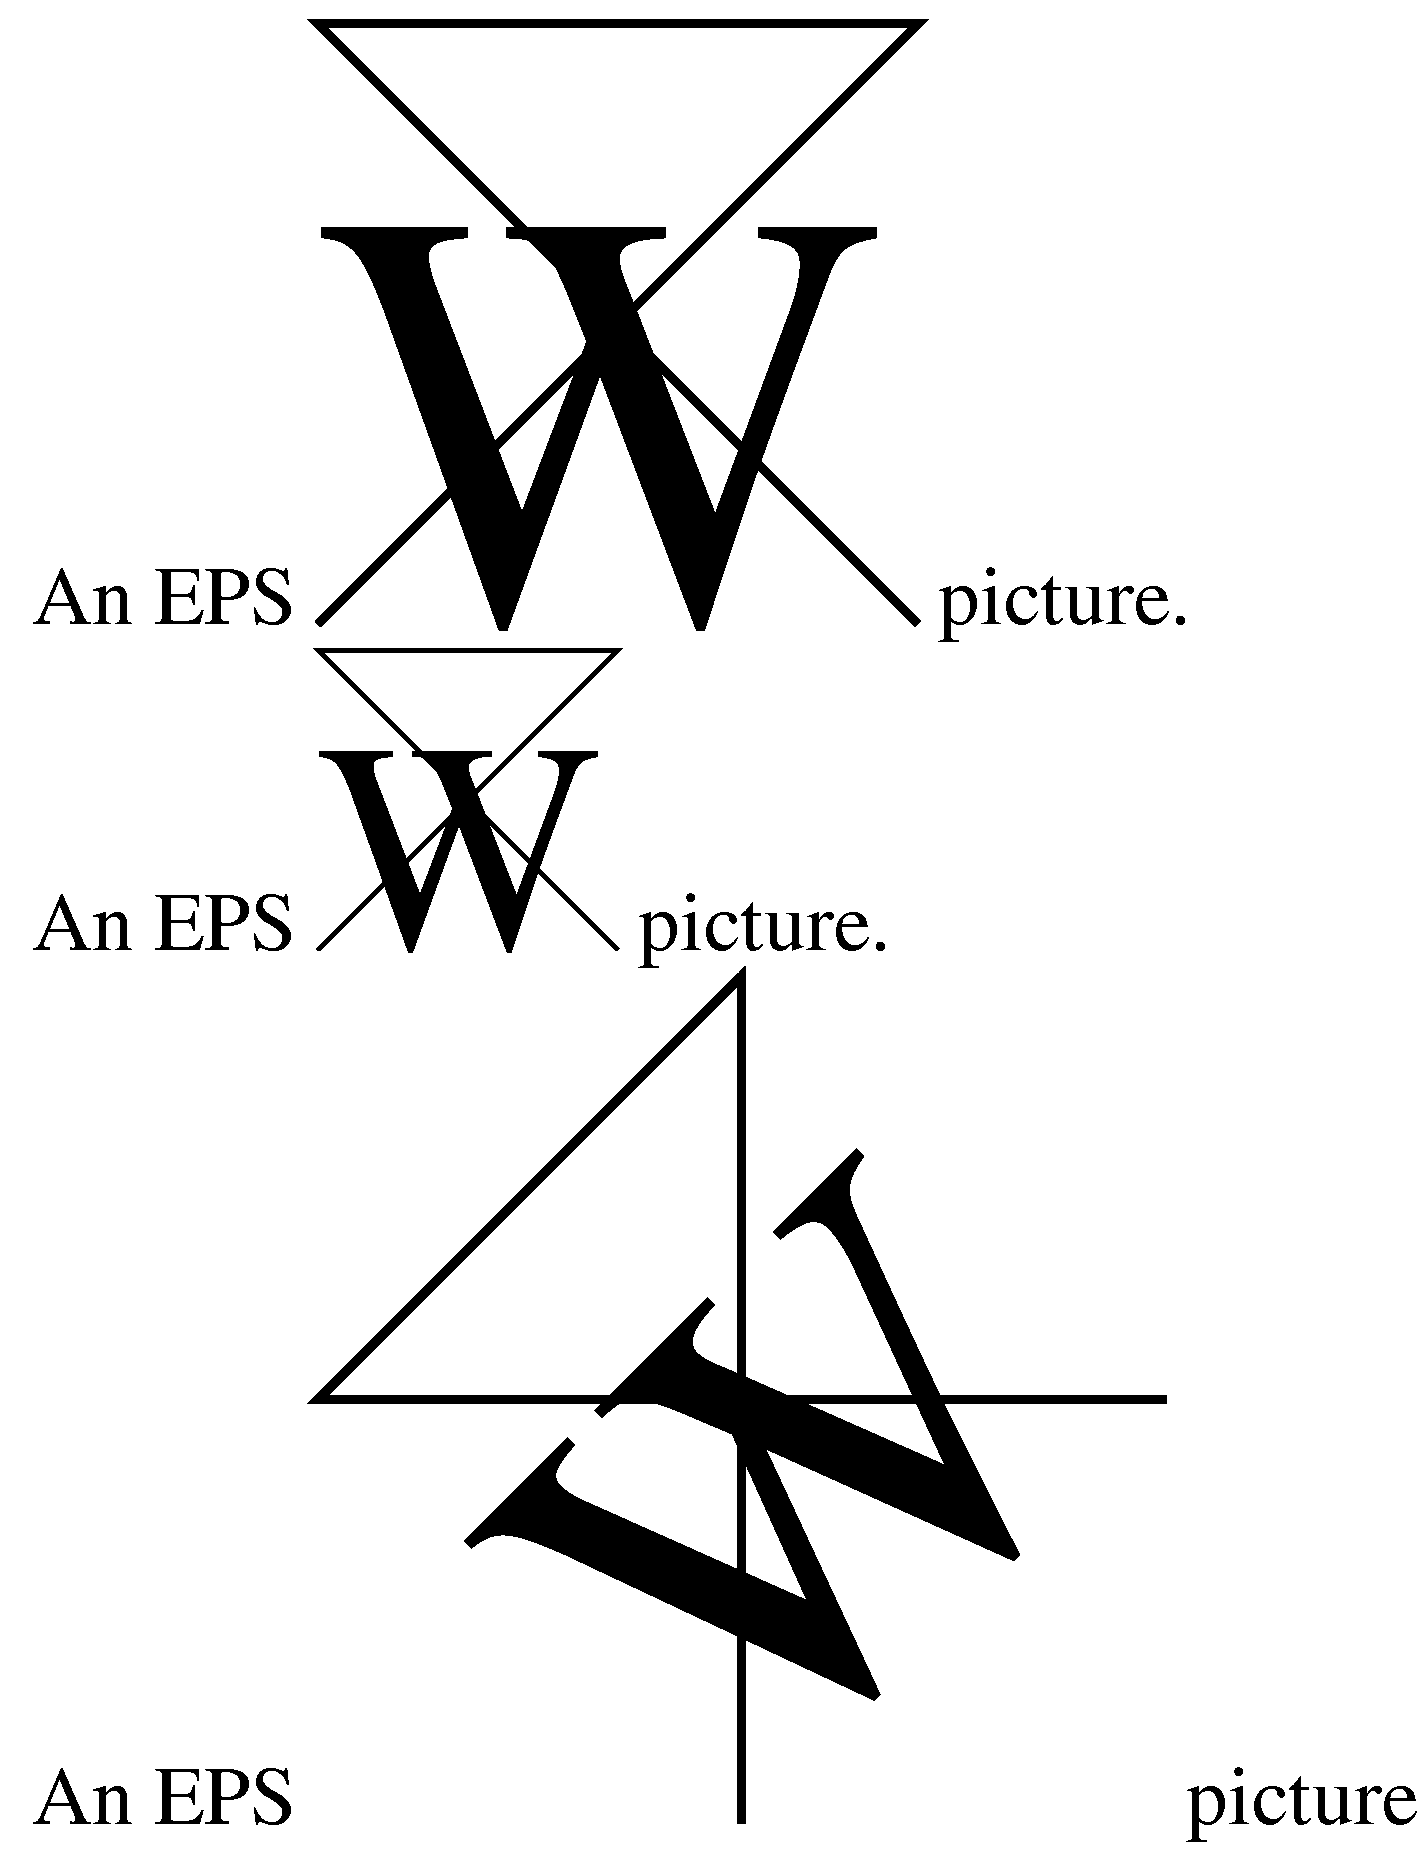
\includegraphics{picture.png}% a full-page picture?
%    \end{textblock*}%
%    \null%
%    \newpage}
% \end{verbatim}
% This inserts a complete page, with some graphic on it, immediately
% after the end of the current page (thanks to Matthias Gloede for
% this technique).
%
% \section{Notes}
% \subsection{Suggestions: Producing large-format posters}
%
% If you are producing a large-format poster, such as A0 size, you
% might want to use Gerlinde Kettl and Matthias Weiser's \cmd|a0poster|
% class, which painlessly deals with the miscellaneous hassles of
% printing to a large-format postscript printer.
%
% I have a collection of suggestions for producing such posters at
% \url{http://purl.org/nxg/note/posters}.
%
% The text on a large poster will typically use a very large font.  It
% can be a hassle to create (or have dvips create) these fonts, and
% they take up a good deal of space on your disk.  You might want to
% investigate the BlueSky/AMS fonts (available at CTAN), which are
% postscript versions of the Computer Modern fonts, and which can
% therefore be scaled arbitrarily.
%
% \subsection{Absolute mode and $\backslash$newpage}
% \label{absolute-newpage}
%
% You can sometimes get rather puzzling behaviour when you use
% |\newpage| in absolute mode.
%
% When using the \Lopt{absolute} option, you will often
% have all of the text on your page inside \Lenv{textblock}
% environments.  In this case, \TeX\ does not believe that you have
% anything on the page at all, and so if you give a |\newpage| command
% to start a second sheet (perhaps you have a particularly generous
% poster space allocation at your conference, or you are filling out a
% form), \TeX\ thinks it is redundant, and ignores it, so that all
% your \Lenv{textblock} environments end up on just one page.  To work
% round this, use |\null\newpage| instead: the |\null| (which produces
% a zero-width box) is enough to persuade
% \TeX\ to respect the page-break.
%
% This happens for the same reason that, also quite surprisingly, two
% |\newline| commands in a row do not produce a blank page.
%
% \subsection{Interactions}
% \label{s:interactions}
%
% Textpos does not appear to get on terribly well with
% Prosper\marginpar{textpos \& prosper} (a
% problem reported by Erik Van Eynde).  This is because
% Textpos in absolute mode places its text onto the page at the last
% moment before the page is shipped out, which will be \emph{after}
% Prosper has rotated the page from portrait to landscape format, so
% that the \Lenv{textblock} contents end up at the correct position on
% the portrait page, but the wrong position on the landscape page.
% This unfortunately means that Textpos in absolute mode is
% incompatible with Prosper.  But all is not lost: since Prosper
% slides start at a consistent point, you can fairly happily use Textpos in
% relative mode as long as the \Lenv{textblock} environment is the
% first thing on the slide.
% \marginpar{\dots \& beamer}
% For a similar reason, you should use the \Lopt{overlay,absolute}
% options with Beamer.\footnote{This is also because the Beamer
% background frame overlays the textpos material, unless the
% \Lopt{overlay} option is used to tell textpos to delay it.
% Thanks to Marius Arenz for useful comments here.}
%
% In general, however, \emph{anything} doing things at |\shipout| time
% (which includes Textpos in absolute mode)
% is going to be in a slightly precarious position
% with respect to anything else which plays games here.
%
% There's also an unfortunate interaction with the \texttt{color}
% package\marginpar{textpos \& color}.  Textpos in absolute mode, and
% the \texttt{pdftex} graphics driver, both squabble over who gets to
% redefine the |\shipout| command: using the |\pagecolor| command with
% \texttt{pdflatex} causes textpos absolute mode to behave
% strangely\footnote{See the \texttt{comp.text.tex} thread `Colour in
% a0 poster' starting 2007 April 3}.  A fix may appear here in time, but
% for the present, there are three workarounds.  The first is to place
% the |\pagecolor{...}| command before |\begin{document}|, which
% causes the redefinitions of |\shipout| to happen in a working
% order.  If this is impossible for some reason, then (as with the
% Prosper workaround above) you can use textpos not in absolute
% mode: if the textblocks are the first printable material on the
% page, then they're anchored at a fixed position, and you should be
% able to use textblocks and |\pagecolor| with \texttt{pdflatex}
% much as normal.  The final possibility is to use \texttt{latex},
% \texttt{dvips} and \texttt{ps2pdf} to produce PDF, since the
% dvips driver happens not to have this problem (thanks to Joris Vankerschaver
% for the initial report, and to Heiko Oberdiek for one of the workarounds).
%
% Gabriel Zachmann suggested having Textpos put a grid on the
% page\marginpar{page grid}, so
% that it is easier to work out \Lenv{textblock} coordinates.  I may
% yet do this, but it may not be necessary, since Rolf Niepraschk's
% \texttt{eso-pic} package can help you create this grid yourself.
% There is a vivid example of using Textpos along with Rolf's
% \texttt{eso-pic} package and the \texttt{calc} package on the
% Textpos web pages, at
% \url{http://purl.org/nxg/dist/textpos}, and an example of how to
% create a grid with TikZ at \url{http://tex.stackexchange.com/a/85088/96}.
%
% Finally, Robert Wenner reported a problem when using Textpos along
% with the \texttt{texdraw} package\marginpar{textpos \& texdraw}, with
% |\move(0,0)| apparently
% making a difference when it should be a no-op.  I haven't worked out
% what's going on here, and further reports of this, ideally with a
% minimal example, would be most welcome.
%
% \subsection{Troubleshooting}
%
% \begin{description}
% \item[Switching to absolute mode with \texttt{$\backslash$TPoptions} doesn't work]
% In order for the \Lopt{absolute} mode to work anywhere, the document
% has to be \emph{started} in absolute mode (see Sect.~\ref{s:changing-options}).
% This is a hard-to-avoid limitation of the way that this mode is implemented.
%
% \item[Error: `Missing number, treated as zero']
% If you give absolute values (that is, values with units) to the
% \Lenv{textblock} environment, then you will be confronted with the
% rather opaque error `Missing number, treated as zero'.  Remember
% that the \Lenv{textblock} environment requires relative sizes, and
% the \Lenv{textblock*} environment requires sizes with units; see
% Sect.~\ref{s:textblock-absolute}.  You get a similar error message
% if you give relative sizes to the \Lenv{textblock*} environment.
%
% \end{description}
%
% \section{History}
% \iffalse @RELEASENOTES@ \fi
% \begin{description}
% \item[\textbf{1.8, 2016 June 5}]\relax 
% \begin{itemize}
% \item Added the |{\TPoptions| command, to switch modes on and
% off within the document.  Various documentation tweaks.
% \item The behaviour of |{\TPMargin| and
% |{\TPMargin*| were somewhat underspecified in versions of
% Textpos before v1.8, and in consequence inconsistently implemented.
% This has now been rationalised, but the change \emph{may} change
% documents which relied on the previous behaviour.
% Thanks to Richard Schreiber for the detailed bug report.
% \end{itemize}
% 
% \item[1.7j, 2014 January 3]\relax 
% Re-released under the LPPL.
% 
% \item[1.7i, 2012 November 10]\relax 
% Bugfix: further change to the way the {color} package is loaded
% (fixes issue 2); now finally fixed?
% 
% \item[1.7h, 2012 June 1]\relax 
% Bugfix: further change to the way the {color} package is loaded.
% Some documentation tweaks.
% Pointers to bitbucket repository.
% 
% \item[1.7g, 2010 September 30]\relax 
% Bugfix: change the way we handle the {color} package not being
% loaded – replacement |{\color| command is now robust.
% Thanks to Joseph Wright for the bugreport.
% Also adjusted documentation of reference points.
% 
% \item[1.7f, 2009 May 28]\relax 
% The change in behaviour introduced in v1.7e is now documented (it
% was unspecified before, and 1.7e didn't commit itself one way or the
% other).
% 
% \item[1.7e, 2009 March 29]\relax 
% Daniel Richard G noted that the order in which textblock contents
% was laid down on the page was counter-intuitive, since one would
% expect that later environments go 'on top of' earlier ones.  This
% order was unspecified before this version, but I've changed this,
% satisfying a principle of least surprise (later ones now go 'on
% top').
% 
% \item[1.7d, 2007 March 30]\relax 
% Axel Sommerfeldt suggested a further alternative approach, even more
% lightweight, and I incorporated a version of that.
% 
% \item[1.7c, 2007 March 29]\relax 
% Giovanni Radilla reported a problem with captions, which meant that the
% captions weren't appearing properly in the list of figures.  Dan
% Luecking and Axel Sommerfeldt analysed the problem precisely, and the
% latter provided code which I've incorporated in this fix.
% 
% \item[1.7b, 2007 March 21]\relax 
% Robert Whittaker reported a problem with |{\TPmargin|,
% which meant that lists and quotations (and other things which
% manipulated |{\leftskip| and |{\rightskip|) were
% not decreasing in size when you set |{\TPmargin| non-zero.
% Fixed.
% 
% \item[1.7a, 2006 September 2]\relax 
% Version 1.7 created an inadvertant dependency on the
% |{{color}| package.  Now, if you do not load that package,
% |{\textblockrulecolour| will have no effect, rather than
% failing.  Textpos will give you a warning in this case, reminding you
% to load the |{{color}| package.
% 
% \item[\textbf{1.7, 2006 August 24}]\relax 
% Added the |{\textblockrulecolour| and
% |{\TPshowboxes{true,false}| commands, to further control the
% display of the rules around the text blocks.
% 
% \item[1.6b, 2006 August 10]\relax 
% Minor documentation fixes
% 
% \item[1.6a, 2005 October 13]\relax 
% The overriding of the figure and table environments now also works
% when there is no previous environment to override.
% 
% \item[\textbf{1.6, 2005 August 30}]\relax 
% Made |{{calc}|-style dimensions to the
% |{{textblock*}| argument work again (so \emph{that's} what
% regression tests are for...).  Override the |{figure| and
% |{table| environments within |{textblock|
% environments, to avoid their surprising and undesirable interaction
% with |{textblock|.
% 
% \item[1.5b, 2005 June 13]\relax 
% The 1.5 release broke the textblock environment's optional
% argument, controlling the position of the reference point within the
% block.  Fixed.
% 
% \item[1.5a, 2005 March 26]\relax 
% Documentation fixes: added a section on the
% interaction between absolute mode and LaTeX's |{\newpage|
% command.
% 
% \item[\textbf{1.5, 2005 March 23}]\relax 
% Implement |{\TPMargin| command, which causes a margin
% to appear round the blocks of text within textblock
% environments.  This makes it easy to use blocks of colour which
% are larger than the block of text by a decent margin, or to put a
% border round textblocks by setting a suitably-sized margin and using
% the |{showboxes| package option.
% 
% \item[\textbf{1.4, 2003 September 7}]\relax 
% Changes in the handling of vertical spacing; inconsistent in some
% circumstances before.  Slight (consequent) change to the algorithm
% which ensures that material is output in absolute mode even when the
% page is otherwise empty.  See README for details.  Version 1.3a will
% remain available for some time in case these fixes break things.
% 
% \item[1.3a, 2003 June 24]\relax 
% Added the |{\textblockcolour| command, to set
% the background colour of text blocks
% 
% \item[\textbf{1.3, 2003 June 24}]\relax 
% (there was a release 1.3, but it was broken, and immediately
% replaced by 1.3a)
% 
% \item[1.2b, 2002 July 1]\relax 
% Works around a bug present in at least one package,
% which leaves box255 holding an hbox at the wrong moment
% 
% \item[1.2a, 2002 April 28]\relax 
% Version 1.2 had an error, which caused a confusing error
% if you gave any fractional part in the arguments to the
% |{{textblock}| environment.  This was fixed in version 1.2a,
% which adds a |{{textblock*}| environment (fully compatible
% with |{calc|), and does not attempt to support calc-style
% expressions in the parameters to the unstarred
% |{{textblock}| environment.
% 
% \item[\textbf{1.2, 2002 April 21}]\relax 
% Rolf Niepraschk |{niepraschk@ptb.de| provided code to
% make textpos compatible with the |{calc| package
% 
% \item[Version 1.1]\relax 
% Released in 1999
% 
% \end{description}
%
% \section{Credits}
%
% Olaf Maibaum, \texttt{Olaf.Maibaum@informatik.uni-oldenburg.de},
% made an elegant improvement to an earlier version of this package,
% by producing the code which I've incorporated here as the `absolute
% mode' (I'd had something like this before, but it was \emph{very}
% kludgy).
%
% Bjoern Pedersen, \texttt{bjoern@poseidon.org.chemie.tu-muenchen.de},
% made the excellent suggestion that the horizontal and vertical
% modules should be independent, and provided code to implement this.
%
% Rolf Niepraschk, \texttt{niepraschk@ptb.de}, provided the code changes
% which made textpos compatible with the \pstyle{calc} package.
%
% Wybo Dekker, \texttt{wybo@servalys.nl}, reported a problem when
% box~255 was (erroneously) not a vbox, and passed on a fix from Hans
% Hagen.
%
% Jenny Maresh and Matthias Jerg independently suggested that it would
% be useful to specify a margin around the block of text in a
% \Lenv{textblock} environment.  That resulted in the |\TPMargin|
% command (after an unconscionably long gestation period).  Rusen Lu
% suggested that one should be able to specify the colours of the box
% borders, and that it would be useful to turn the bordering feature
% on and off within the file.
%
% Axel Sommerfeldt provided elegant code to fix incorrect
% behaviour of |\caption| within the \Lenv{figure} environment.
%
% Section~\ref{s:interactions}, above, lists numerous people who have
% provided problem reports about the interactions between Textpos and
% other packages, and provided suggestions for workarounds and fixes.
%
% Thanks also for general bugreports and other suggestions to
% Jozef Bednarcik,
% Richard G Daniel,
% Wolfgang Fleischer,
% Greg Petriccione,
% Giovanni Radilla,
% Richard Schreiber,
% Brian Stephanik,
% Robert Whittaker,
% Joseph Wright,
% and Joachim Wuttke,
%
% If you've reported a bug or made a suggestion and I haven't credited
% you here, please do accept my apologies, and please let me know.
%
% \section{Example}
%
% Here is a short example file.
%    \begin{macrocode}
%<*example>
\documentclass{article}

\usepackage[absolute]{textpos}

\setlength{\TPHorizModule}{30mm}
\setlength{\TPVertModule}{\TPHorizModule}
\textblockorigin{10mm}{10mm} % start everything near the top-left corner
\setlength{\parindent}{0pt}

\begin{document}

\begin{textblock}{3}(0,0)
This block is 3 modules wide, and is placed with its top left corner
at the `origin' on the page.  Note that the length of the block is not
specified in the arguments -- the box will be as long as necessary to
accomodate the text inside it.  You need to examine the output of the
text to adjust the positioning of the blocks on the page.
\end{textblock}

\begin{textblock}{2}(2,1)
\textblocklabel{block two}
Here is another, slightly narrower, block, at position (2,1) on the page.
\end{textblock}

\begin{textblock}{3}[0.5,0.5](2,3)
This block is at position (2,3), but because the optional argument
[0.5,0.5] has been given, it is the centre of the block which is
located at that point, rather than the top-left corner.
\end{textblock}

\end{document}
%</example>
%    \end{macrocode}
%
% \StopEventually{}

% \section{Implementation}
%    \begin{macrocode}
%<*package>
%    \end{macrocode}
%
%
% \subsection{Options}
%
% Allow the user to switch on display of boxes round the text.
%    \begin{macrocode}
\newif\ifTPshowboxes
\TPshowboxesfalse
\DeclareOption{showboxes}{\TPshowboxestrue}
%    \end{macrocode}
% \dots and switch off printing of text.
%    \begin{macrocode}
\newif\ifTP@showtext
\TP@showtexttrue
\DeclareOption{noshowtext}{\TP@showtextfalse}
%    \end{macrocode}
%
% The user may declare that the positions given to the |\textblock|
% environment are to be absolute on the page, rather than relative to
% the current position.  Relative mode is, and will remain, the
% default, so the \Lopt{relative} option is redundant, but is here for symmetry.
%    \begin{macrocode}
\newif\ifTP@abspos
\TP@absposfalse
\DeclareOption{absolute}{\TP@abspostrue}
\DeclareOption{relative}{\TP@absposfalse}
%    \end{macrocode}
%
% When using the absolute-position mode, the holdbox is placed into
% box~255 in front of the previous contents of box~255.  This is
% normally what you want, but if the page contents have something
% which \emph{obscures} the hold box (for example, a block of opaque
% colour), then the positioned textboxes disappear.  In this case,
% allow the user to specify that the holdbox is to be placed
% \emph{after} the contents of box~255, so that it overlays it rather
% than being overlayed.
% \changes{v1.1c}{1999/03/22}{Added overlay option}
%    \begin{macrocode}
\newif\ifTP@overlay
\TP@overlayfalse
\DeclareOption{overlay}{\TP@overlaytrue}
%    \end{macrocode}
%
% The package can produce some messages reporting on its progress.
% Allow these to be turned off and on explicitly.  The default is
% (currently) on.
% \changes{v1.2}{2002/04/21}{Added verbose and quiet options}
%    \begin{macrocode}
\newif\ifTP@chatter
\TP@chattertrue
\DeclareOption{quiet}{\TP@chatterfalse}
\DeclareOption{verbose}{\TP@chattertrue}
%    \end{macrocode}
%
% That's it.  Now process the options and get on with it.
%    \begin{macrocode}
\ProcessOptions
%    \end{macrocode}
%
% \subsection{Required Packages}
%
% To manipulate |\box255|, this package needs the package
% \texttt{everyshi}, which provides the command |\EveryShipout|.
%    \begin{macrocode}
\ifTP@abspos
  \RequirePackage{everyshi}
\fi
\RequirePackage{keyval}
%    \end{macrocode}
%
% \subsection{Changing options within the text}
%
%    \begin{macrocode}
\define@key{tp}{absolute}{\csname TP@abspos#1\endcsname}
\define@key{tp}{overlay}{\csname TP@overlay#1\endcsname}
\define@key{tp}{verbose}{\csname TP@chatter#1\endcsname}
\define@key{tp}{showboxes}{\csname TPshowboxes#1\endcsname}
\define@key{tp}{showtext}{\csname TP@showtext#1\endcsname}
\def\TPoptions{\setkeys{tp}}
%    \end{macrocode}
%
% \subsection{Other initialisation}
%
% Handle floats.  The following definition of |\TP@xfloat| will be
% used to redefine |\@xfloat| within textblocks.  It has the same
% `interface' as |\@xfloat| -- and in particular, it sets |\@captype|,
% so that |\caption| will still work -- except that it ignores any
% placement specifiers, and doesn't put anything into the |\@currbox|.
% Thus nothing will actually float from here, and thus float out of the
% textblock.
%
% We have to open a box, and set |\@floatpenalty|, because
% |\end@float| expects to close a box; and we don't want to redefine
% |\end@float| because that would required us to redefine
% |\end@dblfloat| as well.  Redefine |\@xympar| to throw an error:
% this means that |\marginpar| is forbidden inside textblocks.  Hmm,
% it also means that it's forbidden even within a minipage -- is that
% a bad thing?
% \changes{1.6a}{2005/10/13}{remove superfluous definitions of thefigure}
% \changes{1.7c}{2007/03/29}{fix caption handling -- code from Axel Sommerfeldt}
% \changes{1.7d}{2007/03/30}{further figure fixes, building on more Axel suggestions}
%    \begin{macrocode}
\def\TP@xfloat#1[#2]{
  \par\def\@captype{#1}%
  \@floatpenalty\z@
  \color@vbox
    \normalcolor
    \vbox\bgroup
}
\def\TP@xympar{
  \PackageError{textpos}
    {You can't use \protect\marginpar\space within a textblock}
    {You're using textpos because you _don't_ want things to float around, yes?}}
%    \end{macrocode}
%
% \subsection{The box handling starts here}
% The text we set will be put into the box |\TP@textbox|.
%    \begin{macrocode}
\newbox\TP@textbox
%    \end{macrocode}
% When the package is invoked in `absolute' mode, the contents of
% |\TP@textbox| are not shipped out immediately, but instead put into the box
% |\TP@holdbox|, which holds the boxes until the page as a whole is
% shipped out (these additions contributed by Olaf Maibaum).
% \changes{v1.1}{1999/02/22}{Introduce holdbox, and absolute/relative modes}
%
% \TeX\ does not call the output routine if there is nothing on the
% page.  To deal with this situation, add code to the end-document
% hook to add a zero-size hbox on the page if |\TP@holdbox| is
% non-empty; the page is no longer empty, so the output routine must
% be called at some point.  The alternative is to add such an hbox at
% the end of every textblock, when in absolute mode.  That solves
% this problem, but introduces others by interfering with vertical spacing.
% (thanks to Bjoern Pedersen for diagnosing this in an old version
% of textpos).
%   \begin{macrocode}
\ifTP@abspos
  \newbox\TP@holdbox            % starts off void
  \AtEndDocument{\ifvoid\TP@holdbox \else \hbox{}\fi}
\fi
%    \end{macrocode}
% All the dimensions (except the optional argument of the textblock
% environment) are in terms of the modules |\TPHorizModule| and
% |\TPVertModule|.
% \changes{v1.1}{1999/02/22}{Distinguish horizontal and vertical modules}
%    \begin{macrocode}
\newdimen\TPHorizModule
\newdimen\TPVertModule
%    \end{macrocode}
%
% \begin{macro}{\TPMargin}
% Macro |\TPMargin| specifies the amount of space left between the
% box, as positioned by the \texttt{textblock}, and the enclosed
% text.  The argument is a dimension, which may as usual be given in
% units of |\TP*Module|.  We signal this to the rest of this package
% by making |\TP@margin| positive (we demand that the argument is
% positive).  The companion dimension |\TP@absmargin| is just the
% absolute value of |\TP@margin|, for convenience.
%    \begin{macrocode}
\newdimen\TP@margin
\TP@margin=0pt
\newdimen\TP@absmargin
\TP@absmargin=0pt
\newcommand{\TPMargin}{%
  \@ifstar\TPMargin@outer\TPMargin@inner
}
\newcommand{\TPMargin@inner}[1]{%
  \TP@margin=#1\relax
  \ifdim\TP@margin < 0pt
    \PackageError{textpos}
      {\protect\TPMargin\space must have a positive argument}
      {\protect\TPMargin\space must have a positive argument}
  \fi
  \TP@absmargin=\TP@margin
}
%    \end{macrocode}
% \end{macro}
% \begin{macro}{\TPMargin*}
% Partnered to this, the |\TPMargin*| command also specifies a margin
% between the text and its enclosing box, but this time the
% \emph{text} is at the position specified by the \texttt{textblock},
% and the box, delimited either by a line or by a panel of colour,
% extends outside this position by an amount specified in the argument
% to this macro.  We signal this to the rest of this package by making
% the margin negative.
%    \begin{macrocode}
\newcommand\TPMargin@outer[1]{%
  \TP@margin=-#1\relax
  \ifdim\TP@margin > 0pt
    \PackageError{textpos}
      {\protect\TPMargin*\space must have a positive argument}
      {\protect\TPMargin*\space must have a positive argument}
  \fi
  \TP@absmargin=-\TP@margin
}
%    \end{macrocode}
% \end{macro}
%
% \begin{macro}{\TPGrid}
% Rather than declare the modules to be specific sizes, they can be
% declared to be proportions of the paper size.  The command
% |\TPGrid{16}{10}| would declare the horizontal module to be a
% sixteenth of the paper size, and the vertical one to be a tenth of
% the paper height.  Set the textblockorigin if the optional arguments
% were provided.
% \changes{v1.1c}{1999/03/09}{Add optional argument to TPGrid}
%    \begin{macrocode}
\def\TPGrid{%
  \@ifnextchar[{\@tempswatrue\TP@Grid}{\@tempswafalse\TP@Grid[0pt,0pt]}}
\def\TP@Grid[#1,#2]#3#4{
  \setlength{\@tempdima}{#1}
  \multiply\@tempdima by 2
  \TPHorizModule=\paperwidth
  \advance\TPHorizModule by -\@tempdima
  \divide\TPHorizModule by #3
  \setlength{\@tempdima}{#2}
  \multiply\@tempdima by 2
  \TPVertModule=\paperheight
  \advance\TPVertModule by -\@tempdima
  \divide\TPVertModule by #4
  \ifTP@chatter
    \typeout{Grid set #3 x #4 = \the\TPHorizModule\space x \the\TPVertModule}%
  \fi
  \ifTP@abspos\if@tempswa \textblockorigin{#1}{#2}\fi\fi
}
%    \end{macrocode}
% \end{macro}
% And use this to initialise initialise the modules to a suitable
% default -- one sixteenth of the paper width and height.
%    \begin{macrocode}
\TPGrid{16}{16}
%    \end{macrocode}
%
% The rules round the boxes are of width |\TPboxrulesize|, and the
% label text within them is |\normalsize|.  For the colour, see
% |\textblockrulecolour|.
%    \begin{macrocode}
\newdimen\TPboxrulesize
\setlength{\TPboxrulesize}{0.4pt}
\def\showtextsize{\normalsize}
%    \end{macrocode}
%
% \begin{macro}{\textblockorigin}
% If we're producing a single page of text, it can be convenient to
% set an origin.  This command may only be used in absolute mode.
%
% First, we need two dimensions, to hold the position of the origin.
% These are relative to the top-left corner of the page, so we need to
% shift them by (1in,1in) to make them relative to the \TeX\ origin.
%    \begin{macrocode}
\ifTP@abspos
  \newdimen\TP@ox
  \newdimen\TP@oy
\fi
%    \end{macrocode}
% The |\textblockorigin| command sets the origin of the page.  It may
% only be called if the package was loaded with the \Lopt{absolute}
% option, so output an error message if that's not the case.
%    \begin{macrocode}
\def\textblockorigin#1#2{%
  \ifTP@abspos
    \TP@ox=-1in    \addtolength\TP@ox{#1}
    \TP@oy=-1in    \addtolength\TP@oy{#2}
    \ifTP@chatter\typeout{TextBlockOrigin set to #1 x #2}\fi
  \else
    \PackageError{textpos}
      {The \protect\textblockorigin\space command\MessageBreak
       may only be used if the package was given\MessageBreak
       the`absolute' option when it was invoked}
      {If you want to use the \protect\textblockorigin\space command, then
         \MessageBreak
       invoke the package with the syntax\MessageBreak
       \protect\usepackage[absolute]{textpos}}
  \fi
  }
%    \end{macrocode}
% \end{macro}
%
% \begin{macro}{\textblocklabel}
% When we're only displaying rules boxes, instead of the text contents
% of the blocks, it's useful to be able to identify which block is
% which.  The contents of |\textblocklabel| are ignored except when
% the \Lopt{noshowtext} option has been used.
%    \begin{macrocode}
\def\textblocklabel#1{\gdef\TP@textblocklabel{#1}}
% (should I use \@bsphack...\@esphack for this?)
%    \end{macrocode}
% \end{macro}
%
% \begin{macro}{\textblockcolour}
% \changes{v1.3}{2003/06/25}{Add textblockcolour}
% \changes{v1.3a}{2003/06/25}{Fix textblockcolour so it works when {color} not loaded}
%    \begin{macrocode}
\def\textblockcolour#1{%
  \@ifundefined{color}%
    {\PackageWarning{textpos}{command textblockcolour used,\MessageBreak
       but {color} package not loaded.\MessageBreak
       Colour changes ignored.}}
    {\gdef\TP@blockcolour{#1}
     \ifx\TP@defaultblockcolour\@undefined
       \gdef\TP@defaultblockcolour{#1}
     \fi
    }}
\def\TP@blockcolour{}           % safe initial default
%    \end{macrocode}
% \end{macro}
% \begin{macro}{\textblockcolor}
% Add a synonym for those who follow Webster's half-hearted spelling reforms.
%    \begin{macrocode}
\let\textblockcolor\textblockcolour
%    \end{macrocode}
% \end{macro}
% \begin{macro}{\tekstblokkulur}
% \dots and one for the hard-core reformers, too.
%    \begin{macrocode}
\let\tekstblokkulur\textblockcolour
%    \end{macrocode}
% \end{macro}
%
% \begin{macro}{\textblockrulecolour}
% We select the colour of the box rules using |\color| (since v1.7).
% However we don't want to depend on the `color' package, so if we're
% showing box rules, and so would be selecting box colours, then give
% a warning but do not fail.  Note the faking of that package's
% commands below.
% \changes{v1.7}{2006/08/24}{Add textblockrulecolour}
%    \begin{macrocode}
\def\textblockrulecolour#1{%
  \@ifundefined{color}%
    {\PackageWarning{textpos}{command textblockrulecolour used,\MessageBreak
       but {color} package not loaded.\MessageBreak
       Colour changes ignored.}}
    {\gdef\TP@rulecolour{#1}}}
\def\TP@rulecolour{black}
%    \end{macrocode}
% Plus spelling-reform variants:
%    \begin{macrocode}
\let\textblockrulecolor\textblockrulecolour
\let\tekstblokroolkulur\textblockrulecolour
%    \end{macrocode}
% \end{macro}
%
% We don't want to create a dependency on the \pstyle{color} package,
% so we shouldn't fail if that package isn't loaded.  Don't check that
% here, since the document, or another package, may load the color
% package later.  Instead, define a command which will create dummy
% no-op definitions for the package commands we use, and invoke this
% just before we invoke any of the color package's commands (see above
% for usage).
%    \begin{macrocode}
\gdef\TP@color[#1]#2{}
\def\TP@checkdummycolorpackage{%
  \@ifundefined{color}%
    {\globaldefs=1
       \DeclareRobustCommand\color[2][]{}%
       \def\color@block##1##2##3{}%
     \globaldefs=0 }{}%
  \global\let\TP@checkdummycolorpackage\relax % don't come here again
}
%    \end{macrocode}
%
% \begin{macro}{\textblock}
% Now define the start of the textblock environment.  Read the first
% argument, and save it for the moment as |\@tempdima|.  If we are
% not in vertical mode, then issue a |\par| to make us so.  The
% environment is documented to create this paragraph break in this
% case, so we don't neet to warn the user about this.
% Then call |\TP@textblock| to read the remaining arguments and start
% off the |\vbox| the body text will be set in.
% \changes{v1.1}{1999/02/22}{Add par here, to put us back into vertical mode}
% \changes{v1.4}{2003/09/05}{Remove warning about par}
%    \begin{macrocode}
\def\textblock#1{%
  \@tempdima=#1\TPHorizModule
  \ifvmode\else
    \ifmmode
      \PackageError{textpos}
        {You cannot use textblock in maths mode}
        {You may use the textblock environment only in \MessageBreak
         vertical mode or horizontal mode (when it triggers a\MessageBreak
         new paragraph).  You cannot use it in maths mode.}
    \else % in horizontal mode
      \par % force us back into vertical mode
    \fi
  \fi
  \@ifnextchar[{\TP@textblock}{\TP@textblock[0,0]}%] bracematch
}
%    \end{macrocode}
% \end{macro}
%
% \begin{macro}{\textblock*}
% |\begin{textblock*}| is a variant of |\begin{textblock}| which takes
% absolute values for its arguments.  It uses |\setlength| throughout,
% and is therefore compatible with the \pstyle{calc} package.
% \changes{1.2a}{2002/04/28}{Added textblock* env}
%    \begin{macrocode}
\def\TP@textblockstar#1{%
  \setlength{\@tempdima}{#1}
  \ifvmode\else
    \PackageWarning{textpos}{environment textblock* not in vertical mode.
      \MessageBreak
      Environment textblock* should not have any text\MessageBreak
      or printable material appearing before it.\MessageBreak
      Alignment may work out wrongly.}%
    \par % force us back into vertical mode
  \fi
  \@ifnextchar[{\TP@textblock}{\TP@textblock[0,0]}%] bracematch
}
\expandafter\let\csname textblock*\endcsname\TP@textblockstar
%    \end{macrocode}
% \end{macro}
%
% \begin{macro}{\TP@textblock}
% Command |\TP@textblock| saves all its arguments in a token list, for
% use in |\TP@endtextblock| later, then it starts a vbox.  Arguments~1
% and~2 are the coordinates of the reference point, as proportions of
% the box's horizontal and vertical size, and arguments~3 and~4 are
% the position of the box in units of the horizontal and vertical modules.
%    \begin{macrocode}
\newtoks\TP@tbargs
\def\TP@textblock[#1,#2](#3,#4){%
  \TP@tbargs={{#1}{#2}{#3}{#4}}%
%    \end{macrocode}
%
% Now (re)define |\@xfloat| and |\@xympar| to be the stub ones defined
% above.  Do this in all cases, even those where the |\figure|
% environment is not defined: if there's no figure environment, this
% will end up otiose rather than wrong, plus this will cope with the
% rather peculiar case where there are some floats defined
% \emph{other} than |\figure|.
%    \begin{macrocode}
  \let\@xfloat\TP@xfloat
  \let\@xympar\TP@xympar
%    \end{macrocode}
%
% Start the |\TP@textbox|, which contains the contents of the textblock.
% Below, let the `textblock' refer to the block of text inside this
% box, and `specwidth' the width provided as argument to the
% \Lenv{textblock} environment.
%    \begin{macrocode}
  \setbox\TP@textbox=\vbox\bgroup
%    \end{macrocode}
% If we're showing boxes, then draw a rule here
%    \begin{macrocode}
    \ifTPshowboxes
      \TP@checkdummycolorpackage
      {\color{\TP@rulecolour}\hrule height0pt depth \TPboxrulesize }%
      \vskip-\TPboxrulesize
    \fi
%    \end{macrocode}
% Cases:
% \begin{itemize}
% \item When |\TP@margin| is zero, then `specwidth', the width of the
% `textblock', and the actual width of |\TP@textbox|, are all equal.
% \item When |\TP@margin| is positive, then `specwidth' is the width
% of |\TP@textbox|, and the `textblock' is narrower (and shorter) than
% this by a margin |\TP@margin| all round (|\hsize| is `specwidth'
% minus 2|\TP@margin|).
% \item When |\TP@margin| is negative, then `specwidth' is the width
% of the `textblock' (|\hsize| is `specwidth'), and |\TP@textbox| is
% wider than this by minus |\TP@margin|.
% \end{itemize}
% Here, when |\TP@margin| is non-zero, we set the `textblock' inside a
% box of appropriate |\hsize|, and put that inside the |\TP@textbox|,
% spaced appropriately (this seems more robust than using
% left- and rightskip, which some environment redefine).
% \changes{v1.7b}{2007/03/21}{Fixed lists inside boxes with non-zero margins}
%    \begin{macrocode}
    \ifdim\TP@margin = 0pt
      \hsize=\@tempdima
      \textwidth\hsize \columnwidth\hsize \linewidth\hsize
    \else
      \vskip\TP@absmargin
      \@tempdimb=\@tempdima % \@tempdimb is outer box width
      \hsize=\@tempdima     % \hsize is inner box width
      \ifdim\TP@margin < 0pt
        \advance\@tempdimb by 2\TP@absmargin % bigger box
      \else
        \advance\hsize by -2\TP@absmargin    % narrower content
      \fi
      \hbox to \@tempdimb\bgroup
        \hskip\TP@absmargin\vbox\bgroup
          \textwidth\hsize \columnwidth\hsize \linewidth\hsize
    \fi
  }
%    \end{macrocode}
% \end{macro}
%
% \begin{macro}{\endtextblock}
% \begin{macro}{\endtextblock*}
% We have two slight variants of the end-block code, depending on
% whether we're in a |{textblock}| or a |{textblock*}| environment.
% The |\if@tempswa| set here is tested below, in |\TP@endtextblock|.
% \changes{1.2a}{2002/04/28}{Added commonendtextblock, and starred variant}
%    \begin{macrocode}
\def\endtextblock{\global\@tempswatrue\TP@commonendtextblock}
\@namedef{endtextblock*}{\global\@tempswafalse\TP@commonendtextblock}
%    \end{macrocode}
% \end{macro}
% \end{macro}
%
% \begin{macro}{\TP@commonendtextblock}
% At the end of the environment, draw the matching horizontal rule
% (if we're showing boxes),
% and finish off the vbox begun in |\TP@textblock|.  Then call
% |\TP@endtextblock| with the arguments we saved in the token register
% in |\TP@tbargs|.
%
% To manipulate the spacing around textblocks, we want to save the
% |\prevdepth| quantity in |\TP@prevdepth|.
%    \begin{macrocode}
\newdimen\TP@prevdepth
%    \end{macrocode}
%
% Now we can handle the end of the textblock.  When |\TP@margin| is
% non-zero, include a final skip which is the size of the absolute
% value of this margin.
%    \begin{macrocode}
\def\TP@commonendtextblock{%
    \ifdim\TP@margin = 0pt
      \relax
    \else
      \egroup % end of inner vbox
      \hskip\TP@absmargin % (just \hfil would work here, too)
      \egroup % end of inner hbox
      \vskip\TP@absmargin
    \fi
    \ifTPshowboxes
        \vskip-\TPboxrulesize
        {\color{\TP@rulecolour}\hrule depth 0pt height \TPboxrulesize}%
    \fi
    \egroup % end of \TP@textbox
%    \end{macrocode}
%
% Control vertical spacing: we need to avoid causing the
% insertion of more space in the case where this \texttt{textblock} is
% between paragraphs of text.  Save the |\prevdepth|, then set it to
% $-1000pt$, suppressing interline glue; then add the zero-size vbox;
% then restore |\prevdepth| to what it was before.  See the discussion
% of interline glue (ie, |\baselineskip| and |\prevdepth|) in
% Chapter~12 (p.~80) of the \TeX book (thanks to Peter M\"unster
% \texttt{<peter@univ-rennes1.fr>} for spotting that I'd got this
% wrong in the previous version).
% \changes{v1.1e}{2001/04/29}{Replace randomly-placed nointerline skip with prevdepth acrobatics, to avoid spacing misfeatures}
% \changes{v1.4}{2003/09/05}{Improve prevdepth calculations, adding TP@prevdepth}
%    \begin{macrocode}
  \TP@prevdepth=\prevdepth
  \prevdepth=-1000pt  % = \nointerlineskip
%    \end{macrocode}
% Finally, call |\TP@endtextblock| to do the work of putting the text
% on the page, directly or indirectly.
%    \begin{macrocode}
  \expandafter\TP@endtextblock\the\TP@tbargs
  }
%    \end{macrocode}
% \end{macro}
%
% \begin{macro}{\TP@endtextblock}
% This is where most of the calculations are. Set temporary dimensions
% a and b to be the coordinates (again, in units of the modules), and
% then adjust them by subtracting the position of the `reference point'
% given by parameters~1 and~2.  These dimensions are pure numbers,
% fractions of the width and height, respectively, of the text block.
% Parameters~3 and~4 indicate where the reference point will be
% positioned.  In the unstarred case (|\if@tempswa| true), these are
% pure numbers, indicating dimensions in units of the |\TPHorizModule|
% and |\TPVertModule| respectively; in the starred case (|\if@tempswa|
% false), they're dimensions.
%
% Position the box |\TP@textbox|, which was build up between
% |\TP@textblock| and |\endtextblock|, at (x,y)=|(#3,#4)|.
% The point that is so positioned is at |(#1\wd,#2\ht)| of
% |\TP@textbox|, so that |(#1,#2)| =(0,0) means top left.
%
% If we're in the absolute-position mode, then we need to make further
% adjustments to these dimensions.
%
% Below, |\@tempdima| and |\@tempdimb| are the $x$- and
% $y$-coordinates of the framebox.
% \changes{v1.5b}{2005/06/13}{Fixed control of reference point, broken in 1.5}
% First, we set these coordinates to be |(#3,#4)|.
%    \begin{macrocode}
\def\TP@endtextblock#1#2#3#4{%
  \if@tempswa % modular/unstarred endtextblock
    \@tempdima=#3\TPHorizModule
    \@tempdimb=#4\TPVertModule
  \else % absolute/starred endtextblock
    \setlength{\@tempdima}{#3}
    \setlength{\@tempdimb}{#4}
  \fi
%    \end{macrocode}
% Next, we adjust them so that the position |(#1,#2)| is at this
% coordinate.  The |\TP@textbox| is the box including the lines
% \emph{and} margin.
%
% Case 1: |\TP@margin| is negative: the `textblock' is `specwidth'
% wide, and box |\TP@textbox| is wider and deeper than
% the `specwidth', by |\TP@margin| all round; we want the position
% |(#1,#2)| to be fractions of the textblock size, not |\TP@textbox|
%    \begin{macrocode}
  \ifdim\TP@margin < 0pt
    \advance\@tempdima \TP@margin
    \advance\@tempdimb \TP@margin
    \@tempdimc=\wd\TP@textbox
    \advance\@tempdimc 2\TP@margin % now \@tempdimc is width of textblock
    \multiply\@tempdimc #1
    \advance\@tempdima -\@tempdimc
    \@tempdimc=\ht\TP@textbox
    \advance\@tempdimc 2\TP@margin % now \@tempdimc is height of textblock
    \multiply\@tempdimc #2
    \advance\@tempdimb -\@tempdimc
%    \end{macrocode}
% Case 2: |\TP@margin| is positive or zero: the |\TP@textbox| is
% `specwidth' in width; the text inside the box is
% narrower than this width; the coordinates |(#1,#2)| are
% fractions of |\TP@textbox| size (ie, `specwidth').
%    \begin{macrocode}
  \else
    \@tempdimc=#1\wd\TP@textbox
    \advance\@tempdima -\@tempdimc
    \@tempdimc=#2\ht\TP@textbox
    \advance\@tempdimb -\@tempdimc
  \fi
%    \end{macrocode}
% FInally, shift the origin if we're in absolute-positioning mode.
%    \begin{macrocode}
  \ifTP@abspos
    \advance\@tempdima by \TP@ox
    \advance\@tempdimb by \TP@oy
  \fi
%    \end{macrocode}
% Then create an hbox inside a vbox, both of size 0pt, in each case
% with the contents prefixed by a skip of the appropriate size, and
% suffixed by |\hss| or |\vss| respectively.  Put the result into the
% temporary box~0
% \changes{v1.3}{2003/06/25}{Add colouring of textblocks}
%    \begin{macrocode}
  \setbox0=\vbox to 0pt{\vskip\@tempdimb
    \hbox to 0pt{\hskip\@tempdima
    \ifx\TP@blockcolour\@empty \else
      {\TP@checkdummycolorpackage
       \color{\TP@blockcolour}%
       \color@block{\wd\TP@textbox}{\ht\TP@textbox}{\dp\TP@textbox}%
      }%
    \fi
    \ifx\TP@defaultblockcolour\@undefined \else
      \global\let\TP@blockcolour\TP@defaultblockcolour
    \fi
    \ifTPshowboxes
      {\color{\TP@rulecolour}\vrule width \TPboxrulesize}%
      \hskip -\TPboxrulesize
    \fi
    \ifTP@showtext
      \box\TP@textbox
    \else
      \vbox to\ht\TP@textbox{%
        \ifTPshowboxes
          {\color{\TP@rulecolour}\hrule depth 0pt height \TPboxrulesize \vskip-\TPboxrulesize}%
        \fi
        \vskip\smallskipamount
        \hbox to\wd\TP@textbox{%
          \ifx\TP@textblocklabel\undefined
            \hbox{}%
          \else
            \hskip\smallskipamount
            \fbox{\showtextsize \TP@textblocklabel}%
            \global\let\TP@textblocklabel\undefined
          \fi
          \hss
        }%
        \vss
        \ifTPshowboxes
          \vskip -\TPboxrulesize
          {\color{\TP@rulecolour}\hrule depth 0pt height \TPboxrulesize}%
        \fi
      }%
    \fi
    \ifTPshowboxes
      \hskip -\TPboxrulesize
      {\color{\TP@rulecolour}\vrule width \TPboxrulesize}%
    \fi
    \hss}%
  \vss
  }%  end of box0
%    \end{macrocode}
% Now switch behaviour depending on whether or not we're in the
% absolute-position mode.  If we are, then add the newly-constructed
% box 0 to (the end of) the holdbox.  The order matters in some
% (many?, all?) circumstances, since this way means that later
% textblock environments go `on top of' earlier ones, which is
% generally more intuitive.  I \emph{think} this would be true for all
% drivers.  Does this have some interaction with the \Lopt{overlay}
% option, and if so, should it be coupled to that?  I haven't
% documented this one way or the other, and I think that ambiguity is
% probably useful.
%    \begin{macrocode}
  \ifTP@abspos
    \global\setbox\TP@holdbox\vbox{%
      \unvbox\TP@holdbox
      \box0
    }%
%    \end{macrocode}
% Else, place the box on the page immediately, and restore the value
% of the quantity |\prevdepth| to what it was before we started
% accumulating material for the textblock.  This will mean (a) that
% we can list several textblock environments one after another, and have them
% all offset from the same point, and (b) that we are invisible with
% respect to any |\parskip| or |\baselineskip| calculations that were
% relevant at the time we started the textblock.
%    \begin{macrocode}
  \else
    \box0
    \prevdepth=\TP@prevdepth
  \fi
  }%
%    \end{macrocode}
% \end{macro}
%
% Finally, and only if we are in the absolute-position mode, set up
% the output routine with |\EveryShipout|, and set the textblockorigin
% to the (default) upper-left corner of the paper.  Respect the
% \Lopt{overlay} option by putting the |\TP@holdbox| contents
% \emph{after} the |\@cclv| contents, putting the latter into a size-0
% box (could this cause a problem with spacing?  I don't think so, at
% this stage).
%
% Box 255 should be either a vbox or void (see \TeX Book pp.~125
% or~253), but if it is an hbox, because some package has misbehaved,
% then we ought to try not to simply collapse.  Work round this by
% testing explicitly whether box~255 is a vbox or not.
% \changes{v1.2b}{2002/07/01}{Defend against box 255 not being a vbox}
%    \begin{macrocode}
\ifTP@abspos
  \ifTP@overlay
    \EveryShipout{%
      \global\setbox\@cclv\vbox{%
        \vbox to 0pt{\ifvbox\@cclv \unvbox\@cclv \else \box\@cclv \fi \vss}%
        \unvbox\TP@holdbox      % TP@holdbox is now void
      }
    }%
  \else
    \EveryShipout{%
      \global\setbox\@cclv\vbox{%
        \unvbox\TP@holdbox
        \ifvbox\@cclv \unvbox\@cclv \else \box\@cclv \fi
      }%
    }%
  \fi
  \textblockorigin{0pt}{0pt}%
\fi
%    \end{macrocode}
% Done!
%    \begin{macrocode}
%</package>
%    \end{macrocode}
%
% \Finale
%
\endinput
